\documentclass[ngerman, 12pt,parskip=half]{scrartcl}

\usepackage[utf8]{inputenc}
\usepackage[T1]{fontenc}
\usepackage{nicefrac}
\usepackage{csquotes}
\usepackage{booktabs}
\usepackage[left=3cm,right=4cm,top=3cm,bottom=3cm]{geometry}
%\usepackage[]{mathpazo,palatino}
\usepackage{fourier}
\usepackage{microtype}
\usepackage{tikz}
\usepackage{pgfplots}
\usepackage{siunitx}
\usepackage{subcaption}
\usepackage{mdframed}

\definecolor{mygray}{rgb}{0.9,0.9,0.9}

\newmdenv [linecolor=black,backgroundcolor=mygray,  frametitle=Anmerkung,leftmargin=0.5cm,rightmargin=0.5cm]{infobox}


\usepackage{listings}

\lstset{literate=%
    {Ö}{{\"O}}1
    {Ä}{{\"A}}1
    {Ü}{{\"U}}1
    {ß}{{\ss}}1
    {ü}{{\"u}}1
    {ä}{{\"a}}1
    {ö}{{\"o}}1
    {~}{{\textasciitilde}}1
}

\definecolor{hellgelb}{rgb}{1,1,0.8}
\definecolor{colKeys}{rgb}{0,0,1}
\definecolor{colIdentifier}{rgb}{0,0,0}
\definecolor{colComments}{rgb}{1,0,0}
\definecolor{colString}{rgb}{0,0.5,0}

\makeatletter
\lstdefinestyle{ausgabe}{
  basicstyle=\ttfamily,%
  backgroundcolor=\color{lightgray}%
}
\makeatother
\lstnewenvironment{ausgabe}{\lstset{style=ausgabe}}{} 


\lstset{%
    float=hbp,%
    basicstyle=\ttfamily\small, %
    identifierstyle=\color{colIdentifier}, %
    keywordstyle=\color{colKeys}, %
    stringstyle=\color{colString}, %
    commentstyle=\color{colComments}, %
    columns=flexible, %
    tabsize=2, %
    frame=single, %
    extendedchars=true, %
    showspaces=false, %
    showstringspaces=false, %
    numbers=left, %
    numberstyle=\tiny, %
    breaklines=true, %
    backgroundcolor=\color{hellgelb}, %
    breakautoindent=true, %
    captionpos=b%
}



% body:            Palatino 10pt
% section titles:  Palatino Bold
% formulas:        Euler-VM
%\usepackage{palatino}
%\usepackage{eulervm}
%\linespread{1.08}  % Palatino needs more leading

% body:            CM Roman 11pt
% section titles:  CM Sansserif Demibold Condensed
% formulas:        CM Math
%\usepackage{ccfonts}
%\setkomafont{sectioning}{\fontfamily{cmss}\fontseries{sbc}\selectfont}


\usepackage[ngerman]{babel}
\usepackage{graphicx}
\usepackage{xcolor}

\usepackage{cancel}


% http://www.latex-community.org/forum/viewtopic.php?f=46&t=21038

\usepackage[bookmarksopen=true,pdfsubject={Statistik},pdftitle={Statistik},pdfauthor={Uwe Ziegenhagen},linkcolor=blue,citecolor=blue,urlcolor=blue,colorlinks=true,pdfproducer={PDFLaTeX},pdfcreator={LaTeX 2e},pdftex,backref]{hyperref}

\usepackage{amsmath,amstext}
\usepackage{attachfile}

\def\qs{\text{QS}(a,b)}
\def\sm{\sum\limits_{i=1}^{n}}
\DeclareMathOperator{\cov}{Cov}
\DeclareMathOperator{\var}{Var}
\DeclareMathOperator{\E}{E}

\title{Einführung in die lineare Regression}
\subtitle{-- DRAFT VERSION--}
\author{Uwe Ziegenhagen}

\begin{document}

\maketitle


Im Rahmen meiner Lehrtätigkeit an Humboldt-Universität zu Berlin und FOM~(Fachhochschule für Oekonomie und Management) durfte ich auch einige Male erklären, wie man die Formeln zur Linearen Regression herleitet. Daraus entstand dann dieses Dokument, das ich hier mit \LaTeX-Quellen zum Download anbiete.

Vielen Dank an diejenigen, die mir Fehler und Ungenauigkeiten im Dokument melden. Am besten dazu ein Issue im github einstellen, ich versuche dann, zeitnah eine neue Version bereitzustellen.

\tableofcontents


\section{Einführung}

Aus der Wikipedia\footnote{\url{https://de.wikipedia.org/wiki/Lineare_Regression}, Abruf: 24.06.2018}: 

\begin{quote}
\enquote{Die lineare Regression, die einen Spezialfall des allgemeinen Konzepts der Regressionsanalyse darstellt, ist ein statistisches Verfahren, mit dem versucht wird, eine beobachtete abhängige Variable durch eine oder mehrere unabhängige Variablen zu erklären. 
Das Beiwort \enquote{linear} ergibt sich dadurch, dass die abhängige Variable eine Linearkombination der Regressionskoeffizienten darstellt (aber nicht notwendigerweise der unabhängigen Variablen).
Der Begriff Regression bzw. Regression zur Mitte wurde vor allem durch den Statistiker Francis Galton geprägt. 
}\end{quote}

Allgemein wird eine metrische Variable \(Y\) betrachtet, die \textit{linear} von ein oder mehreren Variablen \(X_i\) abhängt.
\(Y\) nennt man daher auch die \enquote{abhängige Variable} und die \(X_i\) die \enquote{unabhängigen Variablen}.
Im eindimensionalen Fall -- wenn es nur eine \(X\)-Variable gibt -- spricht man von einer einfachen linearen Regression, in höheren Dimensionen -- wenn es mehrere \(X_i\)-Variablen gibt --  von der multiplen linearen Regression.

\section{Einfache lineare Regression}

Im folgenden nutzen wir die Werte aus Tabelle \ref{tab:werte}, um an ihnen die einfache lineare Regression zu erklären.
Die Zahlen könnten beispielsweise die verkaufte Menge Cocktails (\(Y\)) in Abhängigkeit vom Verkaufspreis (\(X\)) sein.
Die Zahlen wurden so gewählt, dass man gut mit ihnen rechnen kann. 

\begin{center}
\begin{tabular}{cc} \toprule[2pt]
$X$-Wert & $Y$-Wert \\ \midrule
        1 &50\\
        2 &40\\
        3 &45\\
        4 &20\\
        5 &25\\ 
        6 & 15 \\ \bottomrule[2pt]
\end{tabular}
\end{center}
\captionof{table}{Tabelle mit Wertepaaren}\label{tab:werte}\vspace*{1em}

Stellt man die Punkte in einem Streu-Diagramm (auf englisch \enquote{Scatterplot}) wie in Abbildung \ref{fig:scatter} dar, so erkennt man, dass mit steigendem Wert von $X$ die Werte von $Y$ sinken. 

\begin{center}
\vspace*{1em}\begin{tikzpicture}[xscale=1,yscale=0.1,punkt/.style={circle, minimum size = 0.05cm,blue,fill=red}]
%\draw[help lines,yellow,thin] (0,0) grid (9,60);
\draw [->,thick] (0,0) -- (8,0);
\draw [->,thick] (0,0) -- (0,70);
\node  [punkt] (A) at (1,50){};
\node  [punkt] (B) at (2,40){};
\node  [punkt] (C) at (3,45){};
\node  [punkt] (D) at (4,20){};
\node  [punkt] (E) at (5,25){};
\node  [punkt] (F) at (6,15){};
\node  [below] (X) at (3.5,-4){X};
\node  [left] (Y) at (-1,30){Y};
\node  [below] (x1) at (1,0){1};
\node  [below] (x2) at (2,0){2};
\node  [below] (x3) at (3,0){3};
\node  [below] (x4) at (4,0){4};
\node  [below] (x5) at (5,0){5};
\node  [below] (x6) at (6,0){6};
\node  [below] (x7) at (7,0){7};
\node  [left] (y1) at (0,10){10};
\node  [left] (y2) at (0,20){20};
\node  [left] (y3) at (0,30){30};
\node  [left] (y4) at (0,40){40};
\node  [left] (y5) at (0,50){50};
\node  [left] (y6) at (0,60){60};
%\draw[blue, very thick](0,0.8)--(5,4.6);
%\node[punkt] (A) at (9,1){};
%\node[draw] (B) at (8,4){B};
%\draw (A) -- (B);
\end{tikzpicture}
\captionof{figure}{Scatterplot zur Darstellung der X-Y Wertepaare}\label{fig:scatter}\vspace*{1em}
\end{center}

Wenn wir den Zusammenhang dieser Punkte mittels Gerade (also \enquote{linear}) modellieren wollen, unterstellen wir ein Modell der Form: 
   
\begin{equation}
	 Y_i = b + a \cdot x_i + \epsilon_i
\end{equation}

\begin{center}
\begin{tikzpicture}[scale=1,
    punkt/.style={circle, minimum size = 0.05cm,blue,fill=red},
]

\draw[help lines,yellow,thin] (0,0) grid (7,6);
\draw [->,thick] (0,0) -- (7,0);
\draw [->,thick] (0,0) -- (0,6);
\node  [below] (X) at (7,0){X};
\node  [left] (Y) at (0,6){Y};
\draw[blue, very thick](0,1)--(6,4);
\draw[red, very thick](2,2)--(5,2);
\draw[green, very thick](5,2)--(5,3.5);
\draw[magenta, very thick](-0.1,0.1)--(-0.1,0.9);
\node  [left] (b) at (0,1){b};
\node  [right] (y) at (5,2.75){\(\Delta y\)};
\node  [below] (x) at (3.5,2){\(\Delta x\)};

\node  [below] (x) at (5.5,1.5){\( a = \frac{\Delta y}{\Delta x}\)};


\end{tikzpicture}
\captionof{figure}{Grafische Erläuterung}\label{fig:grafisch}
\end{center} 

\begin{itemize}

\item \(b\) ist dabei der Achsenabschnitt, also der Punkt \((0,b)\), an dem die Y-Achse geschnitten wird. 

\item \(a\) hingegen ist der Parameter für die Steigung der Regressionsgeraden, also das Verhältnis von \(\Delta y\) und \(\Delta x\). \(a\) und \(b\) sind für unsere Wertepaare zu bestimmen. 

\item \(\epsilon_i\) steht für die Fehler, den wir bei der Modellierung machen, darauf kommen wir später noch zu sprechen. 

\end{itemize}


Abbildung \ref{fig:grafisch} auf Seite \pageref{fig:grafisch} beschreibt diesen Zusammenhang grafisch.

Wir können wir nun die Regressionsgerade durch die Punkte zeichnen? Abbildung~\ref{fig:geraden} zeigt zwei Beispiele für beliebig gewählte Regressionsgeraden. 
Im linken Teil erkennt man, dass die Gerade schon recht gut zu unseren Punkten passt. 

Im rechten Teil stimmt die Richtung überhaupt nicht, die Gerade impliziert nämlich dass mit steigendem \(X\) die Werte von \(Y\) ebenfalls steigen, also -- angewandt auf unser Beispiel -- bei höherem Preis mehr Cocktails verkauft werden, was normalerweise\footnote{Siehe \url{https://de.wikipedia.org/wiki/Giffen-Paradoxon} für die Ausnahme \enquote{Giffen-Gut}} Quatsch ist.

\begin{figure}[h]
\centering
\subcaptionbox{Mit negativem Anstieg \label{steigneg}}
{
\begin{tikzpicture}[xscale=0.7,yscale=0.1,punkt/.style={circle, minimum size = 0.05cm,blue,fill=red}]
\draw [->,thick] (0,0) -- (8,0);
\draw [->,thick] (0,0) -- (0,70);
\node  [punkt] (A) at (1,50){};
\node  [punkt] (B) at (2,40){};
\node  [punkt] (C) at (3,45){};
\node  [punkt] (D) at (4,20){};
\node  [punkt] (E) at (5,25){};
\node  [punkt] (F) at (6,15){};
\node  [below] (X) at (3.5,-4){X};
\node  [left] (Y) at (-1,30){Y};
\node  [below] (x1) at (1,0){1};
\node  [below] (x2) at (2,0){2};
\node  [below] (x3) at (3,0){3};
\node  [below] (x4) at (4,0){4};
\node  [below] (x5) at (5,0){5};
\node  [below] (x6) at (6,0){6};
\node  [below] (x7) at (7,0){7};
\node  [left] (y1) at (0,10){10};
\node  [left] (y2) at (0,20){20};
\node  [left] (y3) at (0,30){30};
\node  [left] (y4) at (0,40){40};
\node  [left] (y5) at (0,50){50};
\node  [left] (y6) at (0,60){60};
\draw[blue, very thick](1,60)--(6,5);
\end{tikzpicture}}
\subcaptionbox{Mit positivem Anstieg\label{steigpos}}
{
\begin{tikzpicture}[xscale=0.7,yscale=0.1,punkt/.style={circle, minimum size = 0.05cm,blue,fill=red}]
\draw [->,thick] (0,0) -- (8,0);
\draw [->,thick] (0,0) -- (0,70);
\node  [punkt] (A) at (1,50){};
\node  [punkt] (B) at (2,40){};
\node  [punkt] (C) at (3,45){};
\node  [punkt] (D) at (4,20){};
\node  [punkt] (E) at (5,25){};
\node  [punkt] (F) at (6,15){};
\node  [below] (X) at (3.5,-4){X};
\node  [left] (Y) at (-1,30){Y};
\node  [below] (x1) at (1,0){1};
\node  [below] (x2) at (2,0){2};
\node  [below] (x3) at (3,0){3};
\node  [below] (x4) at (4,0){4};
\node  [below] (x5) at (5,0){5};
\node  [below] (x6) at (6,0){6};
\node  [below] (x7) at (7,0){7};
\node  [left] (y1) at (0,10){10};
\node  [left] (y2) at (0,20){20};
\node  [left] (y3) at (0,30){30};
\node  [left] (y4) at (0,40){40};
\node  [left] (y5) at (0,50){50};
\node  [left] (y6) at (0,60){60};
\draw[blue, very thick](1,10)--(6,60);
\end{tikzpicture}}
\caption{Zwei Regressionsgeraden}\label{fig:geraden}
\end{figure}


Da aber eine Einschätzung wie \enquote{recht gut} nicht mathematisch exakt ist, werden wir diesen Punkt ein wenig genauer betrachten.

Betrachten wir dazu Abbildung \ref{fig:geraden2}.
Hier wurden auf der blauen Geraden die Punkte in grün markiert, die eine Regressionsgleichung für den jeweiligen Wert von \(X\) vorhersagt, außerdem wurden die jeweiligen Abstände zwischen dem wahren \(Y\)-Wert und dem geschätzten \(Y\)-Wert (den wir ab jetzt \(\hat Y\) nennen) markiert. 

\begin{tikzpicture}[scale=1,
    pred/.style={circle, minimum size = 0.04cm,blue,fill=green},
    punkt/.style={circle, minimum size = 0.04cm,blue,fill=red}]

\draw [->,thick] (0,0) -- (7,0);
\draw [->,thick] (0,0) -- (0,6);
\draw[blue, very thick](0,6)--(6,2);
\node  [punkt] (A) at (1,1){};
\node  [punkt] (B) at (2,3){};
\node  [punkt] (C) at (3,2){};
\node  [punkt] (D) at (4,5){};
\node  [punkt] (E) at (5,4){};
\node  [pred] (Ap) at (1,5.3333){};
\node  [pred] (Bp) at (2,4.6666){};
\node  [pred] (Cp) at (3,4){};
\node  [pred] (Dp) at (4,3.3333){};
\node  [pred] (Ep) at (5,2.6666){};
\node  [below] (X) at (7,0){X};
\node  [left] (Y) at (0,6){Y};
\node  [below] (suba) at (3.5,0){(a)};
\draw[magenta] (A) -- (Ap);
\draw[magenta] (B) -- (Bp);
\draw[magenta] (C) -- (Cp);
\draw[magenta] (D) -- (Dp);
\draw[magenta] (E) -- (Ep);
\end{tikzpicture}\begin{tikzpicture}[scale=1,
    punkt/.style={circle, minimum size = 0.05cm,blue,fill=red},
    pred/.style={circle, minimum size = 0.05cm,blue,fill=green}]

\draw [->,thick] (0,0) -- (7,0);
\draw [->,thick] (0,0) -- (0,6);
\draw[blue, very thick](0,1)--(6,5);
\node  [punkt] (A) at (1,1){};
\node  [punkt] (B) at (2,3){};
\node  [punkt] (C) at (3,2){};
\node  [punkt] (D) at (4,5){};
\node  [punkt] (E) at (5,4){};
\node  [pred] (Ap) at (1,1.6666){};
\node  [pred] (Bp) at (2,2.3333){};
\node  [pred] (Cp) at (3,3){};
\node  [pred] (Dp) at (4,3.6666){};
\node  [pred] (Ep) at (5,4.3333){};
\draw[magenta] (A) -- (Ap);
\draw[magenta] (B) -- (Bp);
\draw[magenta] (C) -- (Cp);
\draw[magenta] (D) -- (Dp);
\draw[magenta] (E) -- (Ep);
\node  [below] (X) at (7,0){X};
\node  [left] (Y) at (0,6){Y};
\node  [below] (subb) at (3.5,0){(b)};
\end{tikzpicture}
\captionof{figure}{Zwei Regressionsgeraden}\label{fig:geraden2}

Wenn wir die Abweichungen der tatsächlichen \(Y\)-Werte von den geschätzten \(Y\)-Werten als Maß für die Güte der Regression nutzen, dann wird beim Betrachten der beiden Abbildungen schnell klar, dass die Regressionsgerade im linken Bild deutlich schlechter ist als die Regressionsgerade im rechten Bild: die Summe der Abstände zwischen den wahren, roten, Punkten und den durch die Gerade geschätzten Punkten ist deutlich größer.

Aus dieser Tatsache lässt sich ein sehr wichtiger Schluss ziehen: wenn wir diese Summe der Abstände mathematisch \textit{minimieren} könnten, dann würden wir die \textit{optimale}   
Gerade erhalten. 

In Gleichungsform können wir dies wie folgt aufschreiben:

\begin{equation}
S = \sm y_i - \hat{y}_i\label{eq:summedifferenzen}
\end{equation}

In Worten: S ist die Summe aller Differenzen von wahrem und geschätzten $y$-Wert.

Es hat sich als mathematisch sinnvoll herausgestellt, nicht einfach die Summe der Abstände zu minimieren, sondern die Summe der \textit{quadrierten} Abstände. 
Es lässt sich nicht nur leicht damit rechnen, der Kleinste-Quadrate-Schätzer ist auch -- sofern die  Annahmen des klassischen linearen Regressionsmodells nicht verletzt sind -- BLUE (\enquote{Best Linear Unbiased Estimator}). Dazu ein wenig mehr im Anhang unter Abschnitt \ref{sec:blue}. 

Aus Gleichung \ref{eq:summedifferenzen} wird jetzt -- da wir ja die Quadratsumme minimieren wollen -- die folgende Gleichung:

\begin{equation}
QS = \left(\sm y_i - \hat{y}_i\right)^2\label{eq:qabstaende}
\end{equation}

Diese Quadratsumme der Abweichungen ist nur abhängig von den Parametern \(a\) und \(b\) der Regressionsgleichung, daher können wir schreiben:

\begin{equation}
QS(a,b) = \left(\sm y_i - \hat{y}_i\right)^2
\end{equation}%\label{eq:qabstaendea}


Im Folgenden werden wir diese Funktion \textit{partiell ableiten}, um die Gleichungen für die optimalen \(a\) und \(b\) zu ermitteln. 

\section{Herleitung der Parameter-Gleichungen}

Wir schreiben Gleichung \ref{eq:qabstaende} nochmals auf und ersetzen \(\hat y\) durch die Modellgleichung:

\begin{align}\label{eq:1}
\qs	&  = \sm \left(y_i - \hat{y}_i\right)^2\\
								&= \sm \Big(y_i - \overbrace{\big[ax_i+b\big]}^{\hat{y_i}}\Big)^2 \label{eq:2}
\end{align}

Da wir die \textit{optimalen} Werte für die Minimierung dieser Quadratsumme erhalten wollen, bilden wir die partiellen Ableitungen nach \(a\) und \(b\). 

Vorher können wir jedoch Gleichung \ref{eq:2} vereinfachen, denn hier lässt sich zweimal eine Binomische Formel anwenden, was in Gleichung \ref{eq:binform} deutlich wird. Wenn wir den linken Teil des Binoms als \(s\) bezeichnen und den rechten Teil des Binoms als \(t\), dann können wird die zweite Binomische Formel anwenden.

\begin{equation}
\sm \Big( \overbrace{y_i}^{s} - \overbrace{\big[ax_i+b\big]}^{t}  \Big)^2 \label{eq:binform}
\end{equation}

Mit Hilfe der 2. Binomischen Formel\footnote{\quad 2. Binomische Formel: \((s-t)^2 = s^2 -2st + t^2\)} kommen wir von Gleichung \ref{eq:binform} zu Gleichung~\ref{eq:postbinform}:


\begin{equation}
	\qs = \sm \Big( \overbrace{y_i^2}^{s^2} - \overbrace{2y_i (ax_i+b)}^{-2st} + \overbrace{(ax_i +b)^2}^{+t^2}\Big) \label{eq:postbinform}
\end{equation}

Als nächstes können wir noch auf den Ausdruck \(\big(ax_i + b\big)^2 \) die 1. Binomische Formel\footnote{\quad 1. Binomische Formel: \((s+t)^2 = s^2 +2st + t^2\)} anwenden:


\begin{equation}
	\qs = \sm \Big(y_i^2 - 2ax_iy_i - 2by_i + \overbrace{a^2x_i^2}^{s^2} + \overbrace{2abx_i}^{2st} + \overbrace{b^2}^{t^2}\Big)\label{eq:simp}
\end{equation}

Ausgehend von Gleichung \ref{eq:simp} bilden wir jetzt die partiellen Ableitungen nach \(a\) und~\(b\). 

\begin{align}
\frac{\partial\, \qs}{\partial a}	&= \sm \big(-2x_iy_i + 2ax_i^2 + 2bx_i\big) \label{eq:parta1}\\
								&= 2 \sm x_i(-y_i + ax_i + b) \label{eq:parta2a} \\
								&= 2 \sm x_i(ax_i + b -y_i ) \label{eq:parta2} 
\end{align}

\begin{align}
\frac{\partial\, \qs}{\partial b}	&= \sm (-2y_i+2ax_i +2b) \label{eq:partb1}\\
								&= 2 \sm (ax_i + b -y_i) \label{eq:partb2}
\end{align}

Wenn wir Gleichung \ref{eq:partb2} nullsetzen und auflösen, erhalten wir 

\begin{alignat}{3}
2\sm ax_i &+ 2\sm b &&- 2 \sm y_i \quad &&= 0 \\
2\sm ax_i &+ \enskip 2nb &&- 2 \sm y_i \quad &&= 0 \\ 
2nb &= 2 \sm y_i &&- 2\sm ax_i && 
\end{alignat}
%& 2 \sm y_i &&- 2\sm ax_i &&= 2nb

Auflösen nach \(b\) (durch \(2n\) teilen) ergibt zusammen mit der Tatsache, dass das arithmetische Mittel allgemein als \(\bar{x}= \frac{1}{n} \sm x_i \) definiert ist:

\begin{align}
b &= \frac{\sm y_i}{n} - \frac{\sm ax_i}{n} \\
	&= \frac{1}{n} \sm y_i - a \frac{1}{n} \sm x_i \\
	&= \bar{y} - a \bar{x}
\end{align}

Setzen wir nun \(b=\bar{y} - a \bar{x}\) in Gleichung \ref{eq:parta2} ein, erhalten wir

\begin{equation}
	2\sm x_i \big(ax_i + (\bar{y} - a \bar{x}) - y_i\big)=0
	\label{eq:einsetz}
\end{equation}

Durch Ausmultiplizieren und Vereinfachen ergibt sich:

\begin{align}
  0 &= \sm x_i \big(ax_i + (\bar{y} - a \bar{x}) - y_i\big) \\
	&= \sm \big(ax_i^2+x_i(\bar{y}-a\bar{x})-x_iy_i \big) \\
     &= \sm \big(ax_i^2 + x_i\bar{y} - a\bar{x}x_i- x_iy_i \big) \\
     &= \sm \big(ax_i^2 - a\bar{x}x_i + x_i\bar{y} - x_iy_i \big) 
\end{align}

\begin{align}
     &= \sm \big( (ax_i^2 - a\bar{x}x_i) + x_i\bar{y} - x_iy_i \big) \\
     &= \sm \big( ax_i^2 - a\bar{x}x_i \big) + \sm x_i\bar{y} - \sm x_iy_i 
\end{align}

Jetzt subtrahiert man \(\sm x_iy_i\) und addiert \(\sm x_i\bar{y}\), um diese beiden Teile auf die andere Seite der Gleichung zu bekommen. % add/sub ausgetauscht 2020-11-29

\begin{equation}
\sm \left(ax_i^2 -ax_i\bar{x}\right) = \sm x_iy_i - \sm x_i\bar{y} 
\end{equation}

Da \(a\) konstant ist, können wir es vor die Klammer ziehen.

\begin{equation}
a \sm (x_i^2 -x_i\bar{x}) = \sm x_iy_i - \bar{y} \sm x_i 
\end{equation}

Jetzt teilen wir durch \(\sm (x_i^2 -x_i\bar{x})\)

%\begin{equation}
%a \dfrac{\cancel{\sm (x_i^2 -x_i\bar{x})}}{\cancel{\sm (x_i^2 -x_i\bar{x})}}=  \dfrac{\sm x_iy_i - \bar{y} \sm x_i}{\sm (x_i^2 -x_i\bar{x})}
%\end{equation}


\begin{equation}
a =  \dfrac{\sm x_iy_i - \bar{y} \sm x_i}{\sm \big(x_i^2 -x_i\bar{x}\big)} 
\end{equation}

Aus der Definition des arithmetischen Mittels $\bar{x} = \dfrac{1}{n}\sum x_i$ folgt $\sm x_i= n\bar{x}$. Einsetzen ergibt 

\begin{equation}
a =  \dfrac{\sm x_iy_i - \bar{y} n \bar{x}}{ \sm \big( x_i^2 -  x_i \bar{x} \big)}
\end{equation}


Jetzt zerlegen wir die Summe unter dem Bruchstrich in Einzelsummen

\begin{equation}
a =  \dfrac{\sm x_iy_i - \bar{y} n\bar{x}}{\sm x_i^2 - \sm x_i \bar{x}}
\end{equation}

und ziehen \(\bar{x}\) vor das zweite Summenzeichen, denn \(\bar{x}\) ist ja ein konstanter Term:

\begin{equation}
a =  \dfrac{\sm x_iy_i - \bar{y} n\bar{x}}{\sm x_i^2 - \bar{x} \sm x_i}
\end{equation}



Über Formeln zu Varianz und Kovarianz\footnote{Verschiebungssatz: \\ $\cov(X,Y) = \E \left((X - \E(X))(Y - \E(Y)\right)) =\E(X,Y)- \E(X)\E(Y)$ \\ $\var(X)=\E\left(\left(X-\E(X)\right)^2\right)=\E(X^2)-\left(\E(X)\right)^2$} erhalten wir

\begin{equation}
a =  \dfrac{\sm x_iy_i - n\bar{x}\bar{y}}{\sm x_i^2 -n\bar{x}^2} = \dfrac{n \left(\frac{1}{n}\sm x_iy_i - \bar{x}\bar{y}\right)}{ n\left( \frac{1}{n}\sm x_i^2 -\bar{x}^2\right)}  = \dfrac{n\cov(x,y)}{n\var(x)} = \dfrac{\cov(x,y)}{\var(x)}
\end{equation}

 
\begin{infobox}
Die Kovarianz ist definiert als der Erwartungswert der Produkte der Abweichungen zweier Zufallsvariablen von ihren jeweiligen Populations-Mittelwerten. 
Sie ist ein Maß für den \textit{linearen} Zusammenhang, diese Einschränkung ist wichtig.
Eine positive Kovarianz bedeutet, dass sich beide Zufallsvariablen in eine Richtung gemeinsam bewegen (positiv-positiv), eine negative Kovarianz bedeutet, dass sich beide Variablen entgegengesetzt bewegen (positiv-negativ).
\end{infobox}


Damit haben wir die beiden Gleichungen hergeleitet, um die Regressionsgerade zu bestimmen:

\begin{equation}
b=\bar{y} - a \bar{x}
\end{equation}


\begin{equation}
a =  \dfrac{\cov(x,y)}{\var(x)}
\end{equation}

Wie lassen sich die beiden Parameter interpretieren? 

\(a\), die Steigung, gibt den durchschnittlichen Betrag wieder, um den sich \(y\) ändert, wenn \(x\) um eine Einheit verändert wird. 

\(b\) gibt den Betrag von \(y\) an, wenn \(x\) den Wert 0 hat. 

Je nachdem, welche Größen untersucht werden, kann ein \(x\) von 0 sinnvoll interpretiert werden oder nicht. Für eine Untersuchung des  Körpergewichts in Abhängigkeit von der Körpergröße spielt die Körpergröße \(x=0\) sicherlich keine Rolle\ldots    

\section{Beispiel}

\begin{center}
\captionof{table}{Hilfstabelle}
\begin{tabular}{r|cccccc} \toprule
Spalte & 1 & 2 & 3 & 4 & 5 & 6 \\
& $x$	&	$y$	&	$x-\bar{x}$	&	$y-\bar{y}$	&	$(x-\bar{x})(y-\bar{y})$	&	$(x-\bar{x})^2$	\\ \midrule
& 1 &  50 &      -2.5 &      17.5 &                -43.75 &          6.25 \\
& 2 &  40 &      -1.5 &       7.5 &                -11.25 &          2.25 \\
& 3 &  45 &      -0.5 &      12.5 &                 -6.25 &          0.25 \\
& 4 &  20 &       0.5 &     -12.5 &                 -6.25 &          0.25 \\
& 5 &  25 &       1.5 &      -7.5 &                -11.25 &          2.25 \\
& 6 &  15 &       2.5 &     -17.5 &                -43.75 &          6.25 \\
\midrule
$\sum$ & 21 & 195 & & & -122.5 & 17.5 \\ \bottomrule
\end{tabular}
\end{center}

Mit Hilfe der Werte aus der Tabelle lassen sich \(a\) und \(b\) jetzt einfach bestimmen. Hinweis: \(\bar x = 21/6 = 3.5\), \(\bar y = 195/6 = 32.5 \)

\[ a = \frac{\frac{\sum_{i=1}^n \left(x_i-\bar x \right)\left(y_i-\bar y \right)}{6}}{ 
\frac{\sum_{i=1}^6 \left( x_i - \bar x \right)^2}{6}} = \frac{\sum_{i=1}^n\left(x_i-\bar x \right)\left(y_i-\bar y \right)}{\sum_{i=1}^n \left(x_i-\bar x \right)^2}  = \frac{-122.5}{17.5} = -7 \]

Hinweis zu dieser Rechnung: Brüche werden dividiert, indem man mit dem Kehrwert multipliziert: \( \frac{\nicefrac{1}{6}}{\nicefrac{1}{6}}   = \nicefrac{1}{6} \cdot \nicefrac{6}{1}  = 1 \). Für die Berechnung von \(a\) braucht man die Anzahl der Beobachtungen also nicht mehr.

\[ b = \bar y - a\cdot \bar x = 32.5
 - (-7) \cdot 3.5 = 57.0
 \]

Unsere Regressionsgleichung lautet also
\[
y = -7 \cdot x + 57
\]


Mit den gefundenen Werten für unsere beiden Parameter können wir jetzt die Regressionsgerade zeichnen, siehe dazu Abbildung \ref{fig:final} auf Seite \pageref{fig:final}.

\begin{center}
\vspace*{1em}\begin{tikzpicture}[xscale=1,yscale=0.1,punkt/.style={circle, minimum size = 0.05cm,blue,fill=red},
]

%\draw[help lines,yellow,thin] (0,0) grid (9,60);

\draw [->,thick] (0,0) -- (8,0);
\draw [->,thick] (0,0) -- (0,70);

\node  [punkt] (A) at (1,50){};
\node  [punkt] (B) at (2,40){};
\node  [punkt] (C) at (3,45){};
\node  [punkt] (D) at (4,20){};
\node  [punkt] (E) at (5,25){};
\node  [punkt] (F) at (6,15){};

\node  [below] (X) at (3.5,-4){X};
\node  [left] (Y) at (-1,30){Y};

\node  [below] (x1) at (1,0){1};
\node  [below] (x2) at (2,0){2};
\node  [below] (x3) at (3,0){3};
\node  [below] (x4) at (4,0){4};
\node  [below] (x5) at (5,0){5};
\node  [below] (x6) at (6,0){6};
\node  [below] (x7) at (7,0){7};

\node  [left] (y1) at (0,10){10};
\node  [left] (y2) at (0,20){20};
\node  [left] (y3) at (0,30){30};
\node  [left] (y4) at (0,40){40};
\node  [left] (y5) at (0,50){50};
\node  [left] (y6) at (0,60){60};

\draw[blue, very thick](0.5,53.5)--(7,8);
\end{tikzpicture}
\captionof{figure}{Scatterplot mit Regressionsgerade}\label{fig:final}\vspace*{1em}
\end{center}

\section{Maße für die Güte der Linearen Regression}

In diesem Abschnitt möchte ich erläutern, wie man die Stärke des linearen Zusammenhangs und die Güte des linearen Modells bestimmt. Unsere Regressionsparameter \(a\) und \(b\) sind die \textit{optimalen} Modellparameter für die von uns genutzten Daten, aber sie erklären nicht, wie \textit{gut} die Werte der unabhängigen Variablen die Werte unserer abhängigen Variablen erklären.

\subsection{Standardfehler der Schätzung}

Der Standardfehler der Schätzung (auf englisch: standard error of estimate\enquote{SEE}) ist ein Maß dafür, wie stark die tatsächlichen \(Y\)-Werte von den geschätzten Werten (\(\hat{Y}\)) abweichen, er repräsentiert die durchschnittliche Abweichung der beobachteten Werte von der Regressionsgeraden. 

Je kleiner der Standardfehler, desto besser ist die Erklärung durch unser Modell. 

Berechnet wird der Standardfehler für eine Stichprobe wie folgt:

\begin{equation}
\text{SEE} = \sqrt{\frac{1}{N-2} \sum \left(y-\hat{y}\right)^2}
\end{equation}

\(N-2\) steht für die Anzahl der Freiheitsgrade, der Zahl der Beobachtungen minus der Zahl der geschätzten Parameter. In unserem Beispiel haben wir Anstieg und Achsenabschnitt geschätzt, daher beträgt die Zahl der Parameter 2. \clearpage

Hinweis: Berechnet man SEE für eine Grundgesamtheit, dann wird aus \(N-2\) ein \(N\), da keine Parameter mehr geschätzt werden, sondern aus der Population errechnet werden konnten.

Für unser Beispiel ergibt sich SEE daher als:

\begin{center}
\captionof{table}{Berechnung des Standardfehlers}
\begin{tabular}{r|rrrr} \toprule
\(x_i\) & \(y_i\)  & \(\hat{y_i}\) & \(y_i-\hat{y_i}\) & \((y_i-\hat{y_i})^2\) \\ \midrule
1 & 50 & 50 & 0 & 0 \\
2 & 40 & 43 & -3 & 9 \\
3 & 45 & 36 & 9   & 81	\\
4 & 20 & 29 & -9 &  81 \\
5 & 25 & 22 & 3 & 9 \\
6 & 15 & 15 &  0 & 0\\ \midrule
\(\sum\) & & & & 180 \\ \bottomrule
\end{tabular}
\end{center}

\begin{equation}
\text{SEE} = \sqrt{ \frac{1}{4} \cdot 180} = \sqrt{45} = 6.7082
\end{equation}

Wie lässt sich dieser Wert interpretieren? Ich würde es wie folgt beschreiben: \enquote{Im Mittel weicht die prognostizierte Zahl der verkauften Cocktails von der gemessenen Anzahl um ungefähr sieben Stück ab.}

\subsection{Korrelationskoeffizient}

Schauen wir uns zuerst den Korrelationskoeffizienten \(r\) an, auch Bravais-Pearson-Koeffizient  genannt. 

\(r\) misst die Stärke und Richtung des linearen Zusammenhangs zwischen zwei metrischen Variablen. Wichtig ist hier das Wort \enquote{linearen}: \(r\) kann nicht sinnvoll bei nicht-linearen (wie z.\,B. quadratischen) Zusammenhängen genutzt werden.

Für \(r\) gibt es zwei Formeln:

\begin{equation}
r = \frac{\sum_{i=1}^n (x_i - \bar{x})(y_i - \bar{y})}%
{ \sqrt{\sum_{i=1}^n (x_i - \bar{x})^2}  \cdot \sqrt{\sum_{i=1}^n (y_i - \bar{y})^2}}
\end{equation}

\begin{equation}
r = \frac{\sum_{i=1}^n x_iy_i - n\bar{x}\bar{y}}%
{\sqrt{\sum_{i=1}^n x_i^2 - n\bar{x}^2}\cdot \sqrt{\sum_{i=1}^n y_i^2 - n\bar{y}^2}}
\end{equation}

Je nachdem, welche Werte man gegeben hat oder bereits berechnet hat, lässt sich besser mal der einen, mal mit der anderen Gleichung rechnen. Vom Ergebnis her ergeben beide Gleichungen das gleiche Ergebnis.

\(r\) nimmt Werte zwischen -1 und 1 an, der Wert wird wie folgt interpretiert:

\begin{description}
\item [\(r \approx 1\)] positive Korrelation, bei steigenden Werten von X steigen auch die Werte von Y. Beispiele: Größe und Gewicht einer Person, Körpergröße und Schuhgröße, Außentemperatur und Eis-Absatz an der Eisdiele
\item [\(r \approx -1\)] negative Korrelation, bei steigenden Werten von X sinken die Werte von Y. Beispiele: Außentemperatur und Absatz von Glühwein
\item [\(r \approx 0\)] kein linearer Zusammenhang. Beispiel: Körpergröße und Postleitzahl. Hinweis: Ein \(r\) nahe 0 bedeutet nicht, dass es keinen Zusammenhang gibt, er ist halt nur nicht linear. 
\end{description}

Wichtig ist in diesem Zusammenhang, das \(r\) keine Aussagen über die Kausalität trifft! Man könnte vielleicht für die Korrelation der Anzahl der verkauften Smartphones in Hongkong und der Anzahl der verkauften Eistüten in Vancouver ein positives \(r\) messen, kausal gibt es aber zwischen beiden Variablen keinen Zusammenhang.

Mittels Signifikanztest kann man prüfen, ob der errechnet Korrelationskoeffizient tatsächlich signifikant ist oder nur ein Ergebnis des Zufalls unserer Stichprobe ist. Als Hypothesen formulieren wir

\begin{description}
\item[\(H_0\)] Die Korrelation in der Population ist 0 (\(\rho =0\)).
\item[\(H_1\)] Die Korrelation in der Population ist ungleich 0 (\(\rho\not=0\)).
\end{description}

Als Teststatistik für diesen zweiseitigen Test erhalten wir 

\begin{equation}
t = \frac{r\sqrt{n-2}}{\sqrt{1-r^2}}
\end{equation}

\(t\) ist unter der Nullhypothese \(t\)-verteilt mit \(n-2\) Freiheitsgraden. Den kritischen Wert entnehmen wir aus der Tabelle der \(t\)-Verteilung\footnote{z.\,B. von \url{https://www.statistik.tu-dortmund.de/fileadmin/user_upload/Lehrstuehle/Oekonometrie/Lehre/WiSoOekoSS16/tabelletV.pdf}} bei beispielsweise 95\% und \(n-2\)
und lehnen die Nullhypothese ab, wenn unsere Teststatistik kleiner als \(-1\) mal oder größer als der kritische Wert ist.


\subsection{Bestimmtheitsmaß}

Quadriert man \(r\), so erhält man das sogenannte Bestimmtheitsmaß \(R^2\), je nach Literatur auch \enquote{Determinationskoeffizient} bezeichnet. \(R^2\) ist ein Anteilswert, der die erklärte Varianz in das Verhältnis zur Gesamtvarianz setzt. Daraus folgt, dass \(R^2\) Werte zwischen 0 und 1 (0\% und 100\%) annehmen kann. 

Die Formel dafür lautet:

\begin{equation}
R^2 = r^2 = \frac{\sum_{i=1}^n (\hat{y_i} - \bar{y})^2} {\sum_{i=1}^n (y_i - \bar{y})^2}
\end{equation}

Rechnen wir im nächsten Schritt mal \(R^2\) für unser Zahlenbeispiel aus:

\begin{center}
\captionof{table}{Hilfstabelle für die Berechnung von \(R^2\)}
\begin{tabular}{r|lllr} \toprule
i & \(y_i\)  & \(\hat{y_i}\) & \((\hat{y_i} - \bar{y})^2 \)&  \((y_i - \bar{y})^2\) \\ \midrule
1 & 1 &  1.4 & 2.56    & 4.0\\
2 & 3 &  2.2 &  0.64 & 0.0\\
3 & 2 &  3.0 & 0.0     & 1.0\\ 
4 & 5 &  3.8 & 0.64    & 4.0\\ 
5 & 4 &  4.6 & 2.56    & 1.0\\ \midrule
\(\sum\) & & & 6.4 & 10.0\\ \bottomrule
\end{tabular}
\end{center}

Damit ergibt sich

\begin{equation}
R^2 = \frac{6.4}{10.0} = 64 \%
\end{equation}


Zu beachten ist, dass \(R^2\) -- wie \(r\) -- nur eine Aussage über den \textit{linearen} Zusammenhang trifft, für Daten mit einem nicht-linearen Zusammenhang ist es nicht geeignet.

\section{Berechnung mit dem Taschenrechner}

\subsection{Schultaschenrechner}

Moderne (Schul-)Taschenrechner haben alle entsprechende Funktionen eingebaut, um anhand von übergebenen Wertepaaren die Parameter $a$ und $b$ schnell zu bestimmen. Im Folgenden zeigen wir anhand eines Casio Schultaschenrechners vom Typ Casio fx-991DE X CLASSWIZ, wie es funktioniert. 

\begin{enumerate}
	\item Über den \enquote{Menu}-Button wechselt man in das Statistik-Menü und wählt Punkt 2 für das Modell \texttt{y = x + bx}
	\item Es erscheint das Tabellenblatt für die Eingabe der $x$- und $y$-Werte, hier gibt man jetzt alle 12 Werte ein. Mit \enquote{=} wird ein Wert bestätigt, mit den Pfeiltasten wechselt man zwischen den Zellen.
	\item Nach der Eingabe aller Werte drückt man die \enquote{OPTN}-Taste und gelangt in ein Menü.
	\item Mit \enquote{4} kommt man in das \enquote{Regression}-Untermenü, hier zeigt der Rechner dann an:
	
	\begin{itemize}
		\item das Regressionsmodell \texttt{y = a + bx}
		\item den Wert von a: \texttt{a=57}
		\item den Wert von b: \texttt{b=-7}
		\item sowie den Korrelationskoeffizienten \(r\): \texttt{r=-0.909123767}
		\end{itemize}
	
	\item Drückt man wiederholt \texttt{OPTN} und dann die \enquote{3}, so gelangt man in das Menü für die Berechnung der Variablen. Hier zeigt der Rechner die verschiedenen Teilergebnisse wie \(\bar{x}\), \(\sum{x}\), \(\sum{x^2}\), etc.
	\end{enumerate}


\section{Anhang}

\section{\enquote{BLUE} oder der Satz von Gauß-Markov}\label{sec:blue}

Aus der Wikipedia:  Der Satz von Gauß-Markov besagt, dass in einem linearen Regressionsmodell, in dem 

\begin{enumerate}
\item die Störgrößen einen Erwartungswert von null 
\item und eine konstante Varianz haben
\item sowie unkorreliert sind
\end{enumerate}

der Kleinste-Quadrate-Schätzer ein bester linearer erwartungstreuer Schätzer, kurz \enquote{Best Linear Unbiased Estimator} (BLUE) ist. Die drei genannten Punkte sind die Annahmen des klassischen Linearen Regressionsmodells, 


\subsection{Code-Beispiele}



\subsubsection{Python}

\lstinputlisting[language=Python,morekeywords={linregress}]{linreg-01.py}


\begin{ausgabe}
Slope -6.999999999999999
Intercept 57.0
R_value -0.909123767204656
P_value 0.012012484314940097
Std_error 1.6035674514745457
-122.5 17.5
   x   y  x-mean_x  y-mean_y  (x-mean_x)(y-mean_y)  (x-mean_x)^2
0  1  50      -2.5      17.5                -43.75          6.25
1  2  40      -1.5       7.5                -11.25          2.25
2  3  45      -0.5      12.5                 -6.25          0.25
3  4  20       0.5     -12.5                 -6.25          0.25
4  5  25       1.5      -7.5                -11.25          2.25
5  6  15       2.5     -17.5                -43.75          6.25 

Slope:  -7.0 
Intersect:  57.0
\end{ausgabe}

\subsubsection{R}

\lstinputlisting[language=R,morekeywords={lm}]{linreg-01.R}


\begin{ausgabe}
Call:
lm(formula = y ~ x)

Residuals:
         1          2          3          4          5          6 
 9.974e-15 -3.000e+00  9.000e+00 -9.000e+00  3.000e+00  5.112e-15 

Coefficients:
            Estimate Std. Error t value Pr(>|t|)    
(Intercept)   57.000      6.245   9.127 0.000799 ***
x             -7.000      1.604  -4.365 0.012012 *  
---
Signif. codes:  0 '***' 0.001 '**' 0.01 '*' 0.05 '.' 0.1 ' ' 1

Residual standard error: 6.708 on 4 degrees of freedom
Multiple R-squared:  0.8265,	Adjusted R-squared:  0.7831 
F-statistic: 19.06 on 1 and 4 DF,  p-value: 0.01201
\end{ausgabe}

\subsubsection{Microsoft Excel}

Die Excel-Datei in diesem Github-Repo enthält zwei Arbeitsblätter, einmal mit der Berechnung auf traditionelle Weise, einmal mit der Berechnung über die entsprechenden Excel-Formeln \texttt{STEIGUNG} und \texttt{ACHSENABSCHNITT}.



\begin{center}
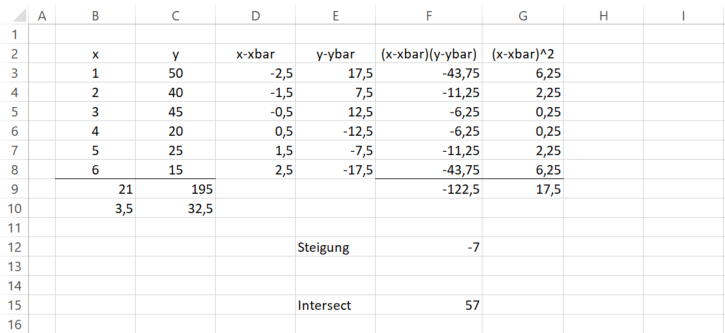
\includegraphics[width=\textwidth]{Excel_manuell}
\captionof{figure}{Manuelle Berechnung in Excel}\label{fig:excelm}
\end{center}



\begin{center}
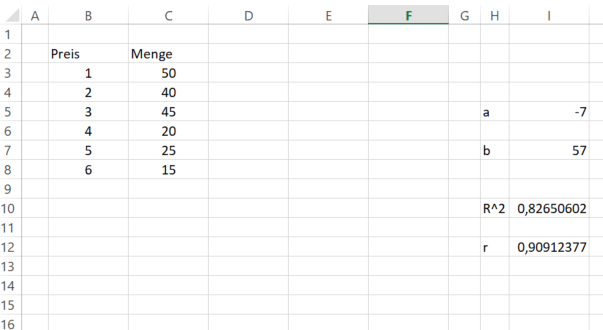
\includegraphics[width=\textwidth]{Excel_Formeln}
\captionof{figure}{Berechnung über Excel-Formeln}\label{fig:excelf}
\end{center}








\section*{Quelldateien}

Dieses Dokument wurde mit \LaTeX, dem freien Textsatzsystem, erstellt. Die Quelldatei dieses Dokuments ist im PDF enthalten, klicken Sie einfach auf das Symbol. Sofern Ihr PDF-Betrachter Attachments unterstützt, sollten Sie auf die Quelldatei zugreifen können.

\begin{tabular}{rl}
  \LaTeX & \attachfile{LinearRegressionPrimer.tex} \\
  Python & \attachfile{linreg-01.py} \\ 
  R & \attachfile{linreg-01.R} \\ 
  Excel & \attachfile{linreg-01.xlsx} \\ 
\end{tabular}



\end{document}


\begin{align}
2\sm ax_i + 2\sm b - 2 \sm y_i &= 0 \\
2\sm ax_i \enskip +\enskip  2nb - 2 \sm y_i &= 0 \\
2nb &= 2\sm y_i - 2 \sm ax_i 
\end{align}

\partial

\stackrel{!}{=}0 


\begin{equation}
	\qs = \sm \Big( \overbrace{y_i^2}^{s^2} - \overbrace{2y_i (ax_i+b)}^{2st} + \overbrace{(ax_i +b)^2}^{t^2}\Big)^2
\end{equation}

Da der Term \((ax_i +b)^2\) der 1. Binomischen Formel entspricht, l�sen wir auch diesen auf: